\begin{figure*}[t]
    \centering
    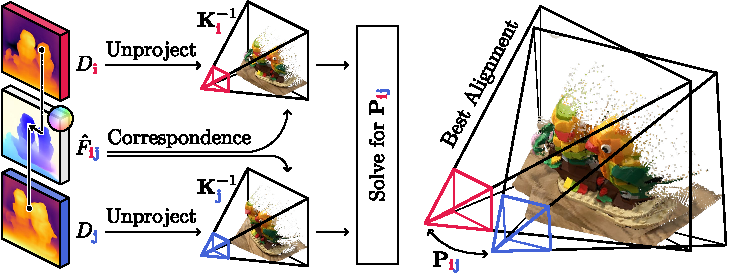
\includegraphics[width=\linewidth,]{figures/procrustes/fig_procrustes_pdf_small.pdf}
    \vspace{-12pt}
    \caption{We solve for the relative poses between consecutive frames using their depth maps, camera intrinsics, and optical flow. To do so, we first unproject their depth maps, then solve for the pose that best aligns the resulting point clouds.}
    \label{fig:procrustes}
    \vspace{-15pt}
\end{figure*}

\section{Supervision via Camera-Induced Scene Flow}
\label{sec:loss}
Given a video sequence, our goal is to supervise per-frame estimates of depth, intrinsics, and pose using known correspondences.
Our method hinges upon the fact that a camera moving through a static scene induces optical flow in image space.
Such optical flow can be computed differentiably from any two images' estimated depths, intrinsics, and relative pose to yield a set of implied pixel-wise correspondences.
These correspondences can then by compared to their known counterparts to yield supervision on the underlying estimates.

Consider a 2D pixel at coordinate $\pixcoord_i \in \mathbb{R}^2$ in frame $i$ of the video sequence. 
Using frame $i$'s estimated depth $\depth_i$ and intrinsics $\ints_i$, we can compute the pixel's 3D location $\pixcoordx_i \in \mathbb{R}^3$.
Then, using the estimated relative pose $\pose_{ij}$ between frames $i$ and $j$, we can transform this location into frame $j$'s camera space.
Finally, we can project the resulting point $\pose_{ij} \pixcoordx_i$ onto frame $j$'s image plane to yield an implied correspondence $\hat\pixcoord_{ij}$.
This correspondence can be compared to the known correspondence $\pixcoord_{ij}$ to yield a loss $\loss$, as illustrated in Fig.~\ref{fig:loss}.
\begin{equation}
    \loss = \| \hat\pixcoord_{ij} - \pixcoord_{ij} \|
    \label{eq:loss}
\end{equation}
\vspace{-25pt}
\myparagraph{Supervision via Dense Optical Flow and Sparse Point Tracks.}
Our known correspondences are derived from two sources: dense optical flow between adjacent frames and sparse point tracks which span longer windows.
Frame-to-frame optical flow ensures that depth is densely supervised, while point tracks minimize drift over time.
We compute correspondences from optical flow $\flow_{ij}$ via $\pixcoord_{ij} = \pixcoord_i + \flow_{ij}[\pixcoord_i]$.
Meanwhile, given a query point $\pixcoord_i$, an off-the-shelf point tracker directly provides a correspondence $\pixcoord_{ij}$ for any frame $j$ where one exists.

\begin{figure*}[t]
    \centering
    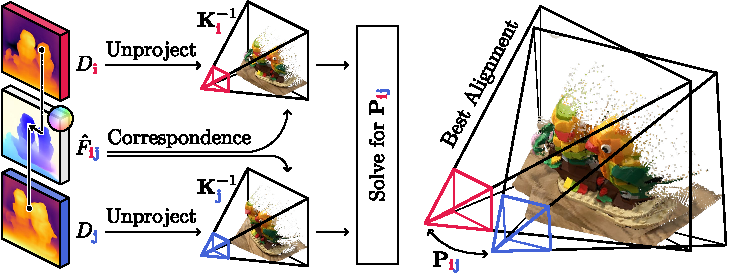
\includegraphics[width=\linewidth,]{figures/procrustes/fig_procrustes_pdf_small.pdf}
    \vspace{-12pt}
    \caption{We solve for the relative poses between consecutive frames using their depth maps, camera intrinsics, and optical flow. To do so, we first unproject their depth maps, then solve for the pose that best aligns the resulting point clouds.}
    \label{fig:procrustes}
    \vspace{-15pt}
\end{figure*}

\myparagraph{Baseline: Pose, Depth and Intrinsics as Free Variables.}
Assuming one uses standard gradient descent optimization, one must decide how to parameterize the estimated depths, intrinsics, and poses.
The simplest choice is to parameterize them as free variables, i.e., to define learnable per-camera intrinsics and extrinsics alongside per-pixel depths.
However, this approach empirically fails to converge to good poses and geometry, as shown in Sec.~\ref{sec:ablations}.


\section{Parameterizing Depth, Pose, and Camera Intrinsics}
\label{sec:reparams}
In this section, we present FlowMap's feed-forward re-parameterization of depth, pose, and camera intrinsics, which uniquely enables high-quality results when using gradient descent. 
Later, in Sec.~\ref{sec:ablations}, we ablate these parameterizations to demonstrate that they lead to dramatic improvements in accuracy.

\myparagraph{Depth Network.} 
If each pixel's depth were optimized freely, two identical or very similar image patches could map to entirely different depths.
We instead parameterize depth as a neural network that maps an RGB frame to the corresponding per-pixel depth. 
This ensures that similar patches have similar depths, allowing FlowMap to integrate geometry cues across frames: if a patch receives a depth gradient from one frame, the weights of the depth network are updated, and hence the depths of all similar video frame patches are also updated.
As a result, FlowMap can provide high-quality depths even for patches which are poorly constrained due to errors in the input flows and point tracks, imperceptibly small motion, or degenerate (rotation-only) motion.

\myparagraph{Pose as a Function of Depth, Intrinsics and Optical Flow.}
\begin{figure*}[t]
    \centering
    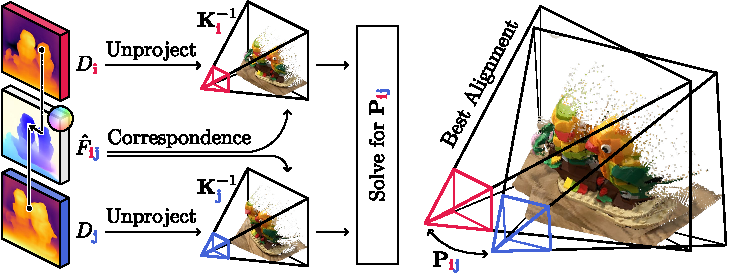
\includegraphics[width=\linewidth,]{figures/procrustes/fig_procrustes_pdf_small.pdf}
    \vspace{-12pt}
    \caption{We solve for the relative poses between consecutive frames using their depth maps, camera intrinsics, and optical flow. To do so, we first unproject their depth maps, then solve for the pose that best aligns the resulting point clouds.}
    \label{fig:procrustes}
    \vspace{-15pt}
\end{figure*}

Suppose that for two consecutive frames, optical flow, per-pixel depths, and camera intrinsics are known.
In this case, the relative pose between these frames can be computed differentiably in closed form.
Following the approach proposed in FlowCam~\cite{smith2023flowcam}, we solve for the relative pose that best aligns each consecutive pair of un-projected depth maps.
We then compose the resulting relative poses to produce absolute poses in a common coordinate system.

More formally, we cast depth map alignment as an orthogonal Procrustes problem, allowing us to draw upon this problem's differentiable, closed-form solution~\cite{choy2020deep}.
We begin by unprojecting the depth maps $\depth_i$ and $\depth_j$ using their respective intrinsics $\ints_i$ and $\ints_j$ to generate two point clouds $\surf_i$ and $\surf_j$.
Next, because the Procrustes formulation requires correspondence between points, we use the known optical flow between frames $i$ and $j$ to match points in $\surf_i$ and $\surf_j$.
This yields $\surf_i^\leftrightarrow$ and $\surf_j^\leftrightarrow$, two filtered point clouds for which a one-to-one correspondence exists.
The Procrustes formulation seeks the rigid transformation that minimizes the total distance between the matched points:
\begin{align}
    \pose_{ij} = \underset{\pose \in \SE(3)}{\argmin} \| \weights^{1/2} (\surf_j^\leftrightarrow - \pose \surf_i^\leftrightarrow )\|_2^2
    \label{eq:procrustes}
\end{align}
The diagonal matrix $\weights$ contains correspondence weights that can down-weight correspondences that are faulty due to occlusion or imprecise flow.
This weighted least-squares problem can be solved in closed form via a single singular value decomposition~\cite{choy2020deep,smith2023flowcam} which is both cheap and fully differentiable.
We further follow FlowCam~\cite{smith2023flowcam} and predict these weights by concatenating corresponding per-pixel features and feeding them into a small MLP. This MLP's parameters are the only other free variables of our model.
For an overview of the depth map alignment process, see Fig.~\ref{fig:procrustes}.

\myparagraph{Camera Focal Length as a Function of Depth and Optical Flow.}

We solve for camera intrinsics by considering a set of reasonable candidates $\ints_k$, then softly selecting among them.
For each candidate, we use our pose solver Eq.~\ref{eq:procrustes} to compute a corresponding set of poses, then use the camera-induced flow loss Eq.~\ref{eq:loss} to compute the loss $\loss_k$ implied by $\ints_k$ and these poses.
Finally, we compute the resulting intrinsics $\ints$ via a softmin-weighted sum of the candidates:
\begin{align}
    \ints = \sum_k w_k \ints_k && w_k = \frac{\exp(-\loss_k)}{\sum_l \exp(-\loss_l)}
\end{align}
To make this approach computationally efficient, we make several simplifying assumptions.
First, we assume that the intrinsics can be represented via a single $\ints$ that is shared across frames.
Second, we assume that $\ints$ can be modeled via a single focal length with a principal point fixed at the image center.
Finally, we only compute the soft selection losses on the first two frames of the sequence.

\myparagraph{Depth as the Only Free Variable in SfM.} FlowMap offers a surprising insight: Given correspondence, SfM can be formulated as solving for per-frame depth maps.
FlowMap yields poses and intrinsics in a parameter-free, differentiable forward pass when given correspondences and depths.
This means that better initializations of FlowMap's depth estimator (e.g., from pre-training) will yield more accurate camera parameters (see Fig.~\ref{fig:prior}).

\begin{figure*}[t]
    \centering
    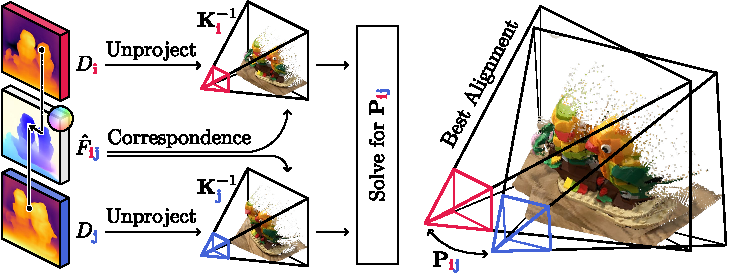
\includegraphics[width=\linewidth,]{figures/procrustes/fig_procrustes_pdf_small.pdf}
    \vspace{-12pt}
    \caption{We solve for the relative poses between consecutive frames using their depth maps, camera intrinsics, and optical flow. To do so, we first unproject their depth maps, then solve for the pose that best aligns the resulting point clouds.}
    \label{fig:procrustes}
    \vspace{-15pt}
\end{figure*}


\section{Implementation and Optimization Details}
\label{sec:optimization}
FlowMap is optimized on each specific scene, achieving convergence between 500 and 5,000 steps using the Adam~\cite{kingma2014adam} optimizer.
Though per-scene optimization is key to achieving high accuracy, we find that exploiting FlowMap's feed-forward nature for pre-training yields an initialization that leads to improved convergence and accuracy, as shown in Fig.~\ref{fig:prior}.
We use RAFT~\cite{raft} and CoTracker V1~\cite{karaev2023cotracker} to compute the optical flow and point tracks that FlowMap uses as input.

\myparagraph{Focal Length Regression.}

While our soft selection approach robustly yields near-correct focal lengths, its performance is slightly worse compared to well-initialized direct regression.
We therefore switch to focal length regression after 1,000 steps, using our softly selected focal length as initialization.

\myparagraph{Memory and Time Requirements.}

FlowMap's complexity in time and memory is linear with the number of input video frames.
During each optimization step, FlowMap recomputes depth for each frame, then derives poses and intrinsics from these depths to generate gradients.
In practice, FlowMap optimization for a 150-frame video takes about 20 minutes, with a peak memory usage of about 36 GB.
Precomputing point tracks and optical flow takes approximately 2 minutes.
Note that FlowMap's runtime could be reduced by early stopping, and its memory usage could be reduced by performing backpropagation on video subsets during each step, but we leave these optimizations to future work.

\myparagraph{Sequence Length and Drift.} 
Since adjacent frames in typical 30 FPS videos usually contain redundant information, we run FlowMap on subsampled videos.
We perform subsampling by computing optical flow on the whole video, then selecting frames so as to distribute the overall optical flow between them as evenly as possible.
With this strategy, we find that an object-centric, full $360^\circ$ trajectory as is common in novel view synthesis papers is covered by about $90$ frames.
We note that FlowMap does not have a loop closure mechanism.
Rather, point tracks provide long-range correspondences that prevent the accumulation of drift in long sequences.
